%\iffalse
\let\negmedspace\undefined
\let\negthickspace\undefined
\documentclass[journal,12pt,twocolumn]{IEEEtran}
\usepackage{cite}
\usepackage{amsmath,amssymb,amsfonts,amsthm}
\usepackage{algorithmic}
\usepackage{graphicx}
\usepackage{textcomp}
\usepackage{xcolor}
\usepackage{txfonts}
\usepackage{listings}
\usepackage{enumitem}
\usepackage{mathtools}
\usepackage{gensymb}
\usepackage{comment}
\usepackage[breaklinks=true]{hyperref}
\usepackage{tkz-euclide} 
\usepackage{listings}
\usepackage{gvv}                                        
\def\inputGnumericTable{}                                 
\usepackage[latin1]{inputenc}                                
\usepackage{color}                                            
\usepackage{array}                                            
\usepackage{longtable}                                       
\usepackage{calc}                                             
\usepackage{multirow}                                         
\usepackage{hhline}                                           
\usepackage{ifthen}                                           
\usepackage{lscape}
\usepackage{circuitikz}
\newtheorem{theorem}{Theorem}[section]
\newtheorem{problem}{Problem}
\newtheorem{proposition}{Proposition}[section]
\newtheorem{lemma}{Lemma}[section]
\newtheorem{corollary}[theorem]{Corollary}
\newtheorem{example}{Example}[section]
\newtheorem{definition}[problem]{Definition}
\newcommand{\BEQA}{\begin{eqnarray}}
\newcommand{\EEQA}{\end{eqnarray}}
\newcommand{\define}{\stackrel{\triangle}{=}}
\theoremstyle{remark}
\newtheorem{rem}{Remark}
\begin{document}

\bibliographystyle{IEEEtran}
\vspace{3cm}

\title{DISCRETE}
\author{EE23BTECH11006 - Ameen Aazam$^{*}$% <-this % stops a space
}
\maketitle
\newpage
\bigskip

\renewcommand{\thefigure}{\theenumi}
\renewcommand{\thetable}{\theenumi}

\vspace{3cm}
\textbf{Question :}
The time-dependent growth of a bacterial population is governed by the equation
\begin{align}
    \frac{dx}{dt}=x\brak{1-\frac{x}{200}}
\end{align}
where $x$ is the population size at time $t$. The initial population size is $x_0=100$
at $x=0$. As $t \rightarrow \infty$, the population size of bacteria asymptotically approaches \ldots.
\hfill{(GATE BM 2023)}

\solution
%\fi
\begin{table}[htbp]
    \centering
    \begin{tabular}{|c|c|c|} \hline
      \textbf{Parameters} & \textbf{Values} & \textbf{Description} \\ \hline
      $t$ &  & Time, Independent variable \\ \hline
      $x(t)$ &  & Population size at any time \\ \hline
      $x(0)$ & $100$ & Initial population \\ \hline
      $h$ &  & Step size \\ \hline
      $x(n)$ &  & Discrete-Time approximation of $x(t)$ \\ \hline
    \end{tabular}
    \vspace{3pt}
    \caption{Parameters}
    \label{tab:x}
\end{table}

The growth equation is given by,
\begin{align}
    &\frac{dx}{dt}=x\brak{1-\frac{x}{200}} \\
    \implies &{dx\brak{t}}{dt}=\frac{1}{200}x\brak{200-x} \\
    \implies &\frac{1}{200}\brak{\int_{0}^{x\brak{t}}\frac{dx}{200-x}+\int_{0}^{x\brak{t}}\frac{dx}{x}}=\int_{0}^{t}\frac{dt}{200} \\
    \implies &-\ln{\brak{200-x}}|_{100}^{x\brak{t}}+\ln{\brak{x}}|_{100}^{x\brak{t}}=t \\
	\implies &\frac{x\brak{t}}{200-x\brak{t}}=e^t \\
    \implies &x\brak{t}=\frac{200}{1+e^{-t}}
\end{align}
We can also express the growth equation as,
\begin{align}
    \implies &\int_{0}^{x\brak{t}}dx=\int_{0}^{t}xdt-\frac{1}{200}\int_{0}^{t}x^2dt
\end{align}
Now approximating by trapezoidal rule of integration between $t_{n-1}$ to $t_n$ with the step size being $h$ we have,
\begin{align}
    \begin{split}
        x\brak{t_n}-x\brak{t_{n-1}}=&\frac{h}{2}\sbrak{x\brak{t_n}+x\brak{t_{n-1}}}- \\
        &\frac{h}{400}\sbrak{x^2\brak{t_n}+x^2\brak{t_{n-1}}}
    \end{split}
\end{align}
Next, replacing $t_{n}=hn$ we get the difference equation,
\begin{align}
    &x\brak{hn}=\frac{-\brak{1-\frac{h}{2}}+\sqrt{\brak{1-\frac{h}{2}}^2+\frac{h}{100}p_1}}{h/200}
\end{align}
Where,
\begin{align}
    p_1=\sbrak{\brak{1-\frac{h}{2}}x\brak{h\brak{n-1}}-\frac{h}{400}x^2\brak{h\brak{n-1}}}
\end{align}
And relabeling $hn\longleftrightarrow n$ we will be having the discrete time equation as,
\begin{align}
    x\brak{n}=\frac{-\brak{1-\frac{h}{2}}+\sqrt{\brak{1-\frac{h}{2}}^2+\frac{h}{100}p_2}}{h/200} \label{eq:A}
\end{align}
Where,
\begin{align}
    p_2=\sbrak{\brak{1-\frac{h}{2}}x\brak{n-1}-\frac{h}{400}x^2\brak{n-1}}
\end{align}
Now, plotting both the differential and the difference equations,
\begin{figure}[h]
    \centering
    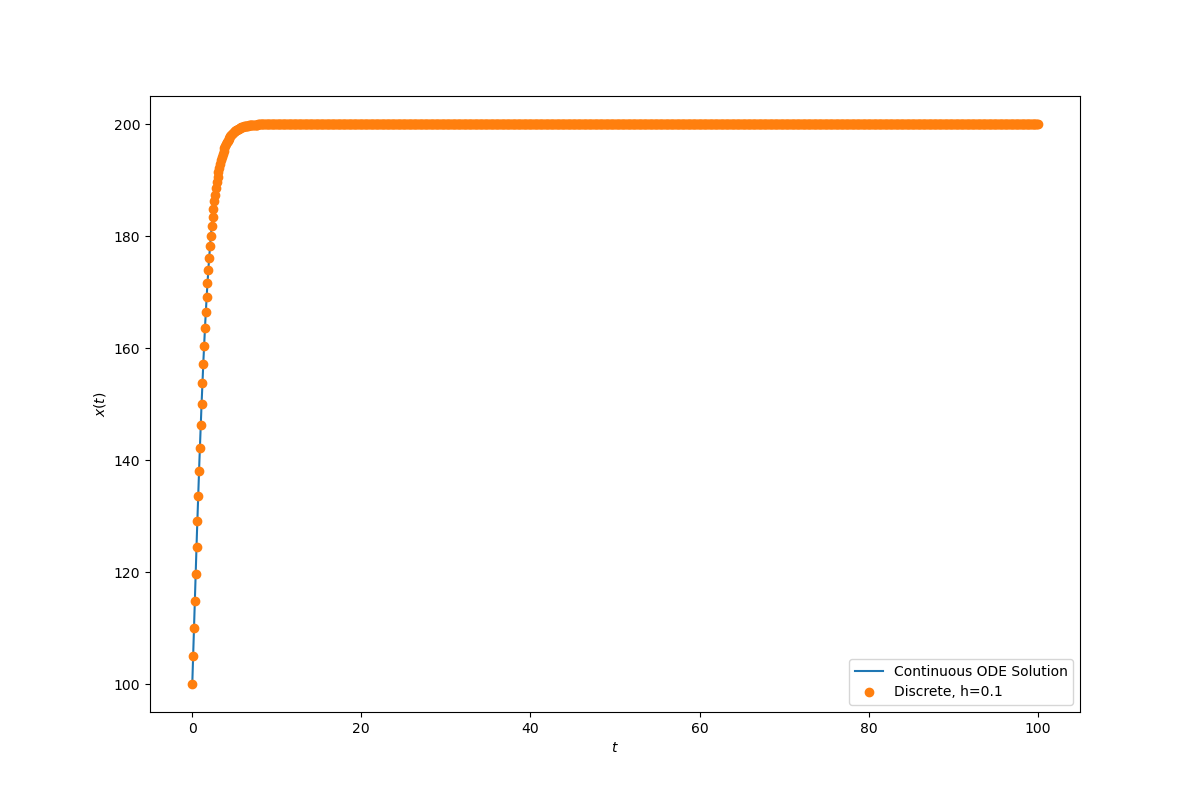
\includegraphics[width=\columnwidth]{figs/diff.png}
    \caption{Approximation in Discrete-Time}
\end{figure}
\newline
As we can see the discrete time plot is following the actual curve, which means \eqref{eq:A} is indeed a good approximation of the original continuous-time equation.
\newline
And the population size approaches to 200 as $t \rightarrow \infty$.
\end{document}
